\chapter{Implementasi dan Pengujian}
\label{chap:implementasiPengujian}

Bab ini terdiri atas dua bagian, yaitu Implementasi Perangkat Lunak dan Pengujian Perangkat Lunak. Bagian implementasi berisi penjelasan lingkungan pengembangan perangkat lunak dan hasil implementasi. Sedangkan bagian pengujian berisi hasil pengujian fungsional dan eksperimental terhadap perangkat lunak yang telah dibangun.

\section{Implementasi}
\label{sec:implementasi}

\subsection{Lingkungan Implementasi}
		\label{sec:lingkungan_implementasi}
			Implementasi perangkat lunak ini dilakukan di dua buah komputer. Implementasi pertama dilakukan pada komputer peneliti untuk keperluan pengujian fungsional. Komputer tersebut memiliki spesifikasi sebagai berikut:
				\begin{enumerate}
					\item Processor: 3.20Ghz 
					\item RAM: 4.00 GB DDR3	
					\item Sistem Operasi: Windows 8.1 Pro 64-bit 
					\item Versi Java: 1.8.0\_40
				\end{enumerate}
				Implementasi kedua dilakukan pada komputer server yang terhubung dengan jaringan FTIS untuk keperluan pengujian eksperimental. Komputer tersebut memiliki spesifikasi sebagai berikut:
				\begin{enumerate}
					\item Processor: 2.66Ghz 
					\item RAM: 4.00 GB DDR2	
					\item Sistem Operasi: Ubuntu server amd-64 
					\item Versi Java: 1.8.0\_66
				\end{enumerate}

\subsection{Hasil Implementasi}
				Hasil implementasi berupa aplikasi berbasis web yang menggunakan \textit{framework} Bootstrap\footnote{\url{http://getbootstrap.com/}, diakses 20 November 2015}. Aplikasi dapat diakses pada jaringan FTIS dengan URL \url{http://studentportal-if.ftis.unpar:9000}. Aplikasi Informatika Student Portal terdiri dari lima halaman antara lain:
			\begin{enumerate}	 
				\item\textbf{Halaman \textit{Login}}\\
				Halaman \textit{login} digunakan pengguna untuk masuk ke dalam aplikasi. Pada halaman ini, pengguna dapat melakukan \textit{login} dengan mengisi \textit{email} pada kolom \textit{email} dan \textit{password} pada kolom \textit{password} kemudian mengklik tombol login. Tangkapan layar dari halaman \textit{login} dapat dilihat pada Gambar \ref{fig:5_hasil_login}.
					\begin{figure}[H]
						\centering
						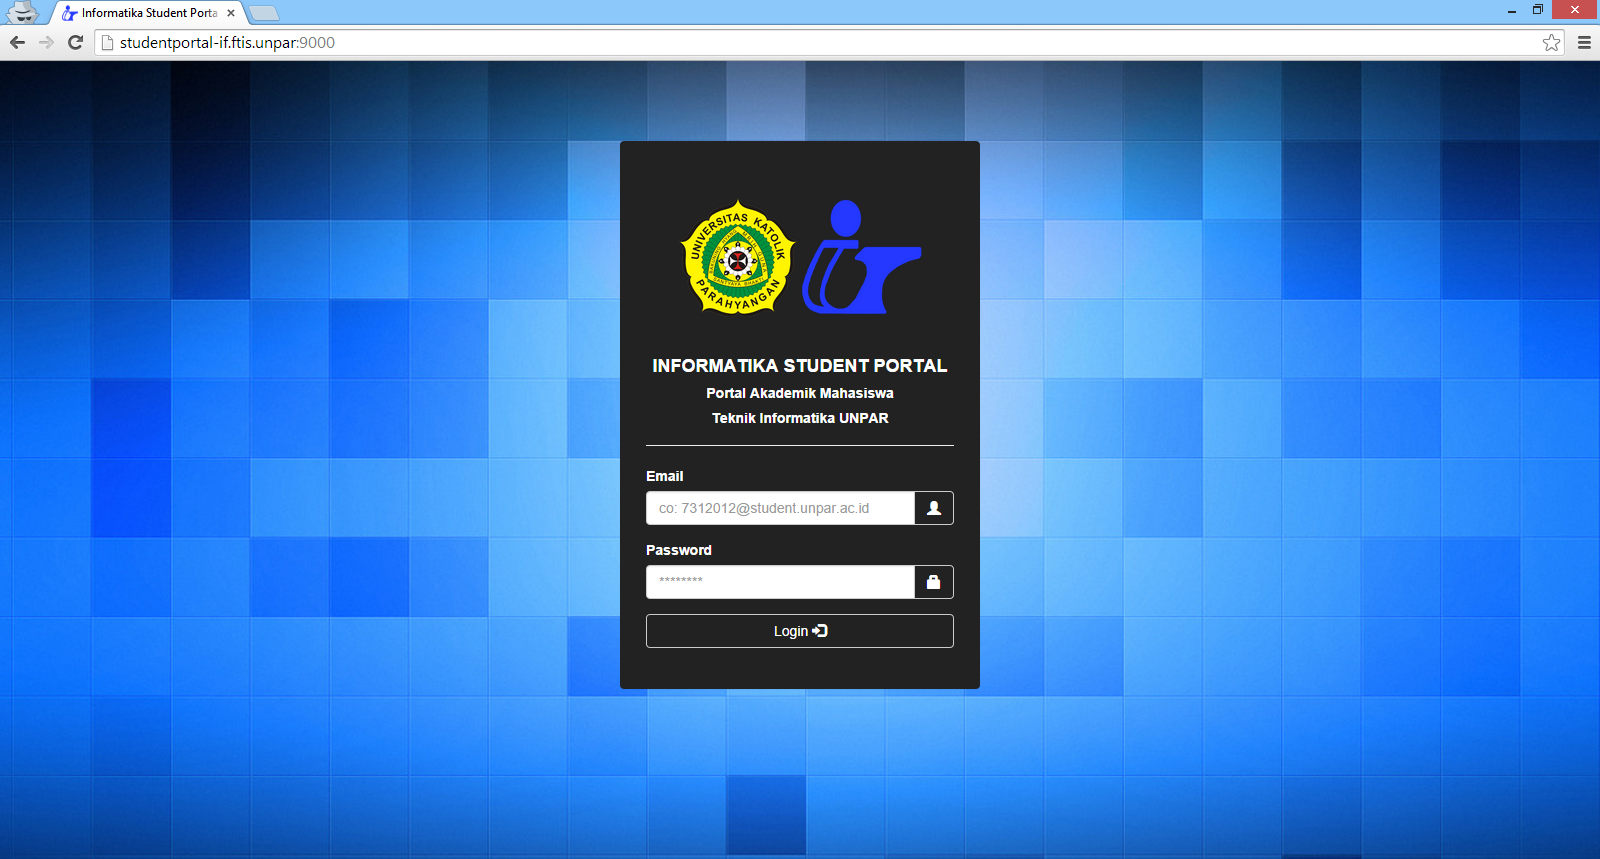
\includegraphics[scale=0.34]{Gambar/hasil_login}
						\caption{Halaman \textit{Login}} 
						\label{fig:5_hasil_login}
					\end{figure}
					
				\item\textbf{Halaman \textit{Home}}\\
				Halaman utama merupakan halaman yang pertama kali dituju setelah melakukan \textit{login}. Halaman utama menampilkan identitas pengguna dan \textit{link} menuju kode sumber aplikasi Informatika Student Portal. Pada halaman ini juga terdapat \textit{sidebar menu} yang diperoleh dari \textit{template} StartBootstrap\footnote{\url{http://startbootstrap.com/}, diakses 20 November 2015}. \textit{Template} tersebut juga digunakan pada halaman prasyarat mata kuliah, jadwal kuliah, dan data akademik. Tangkapan layar dari halaman utama dapat dilihat pada Gambar \ref{fig:5_hasil_utama}.
					\begin{figure}[H]
						\centering
						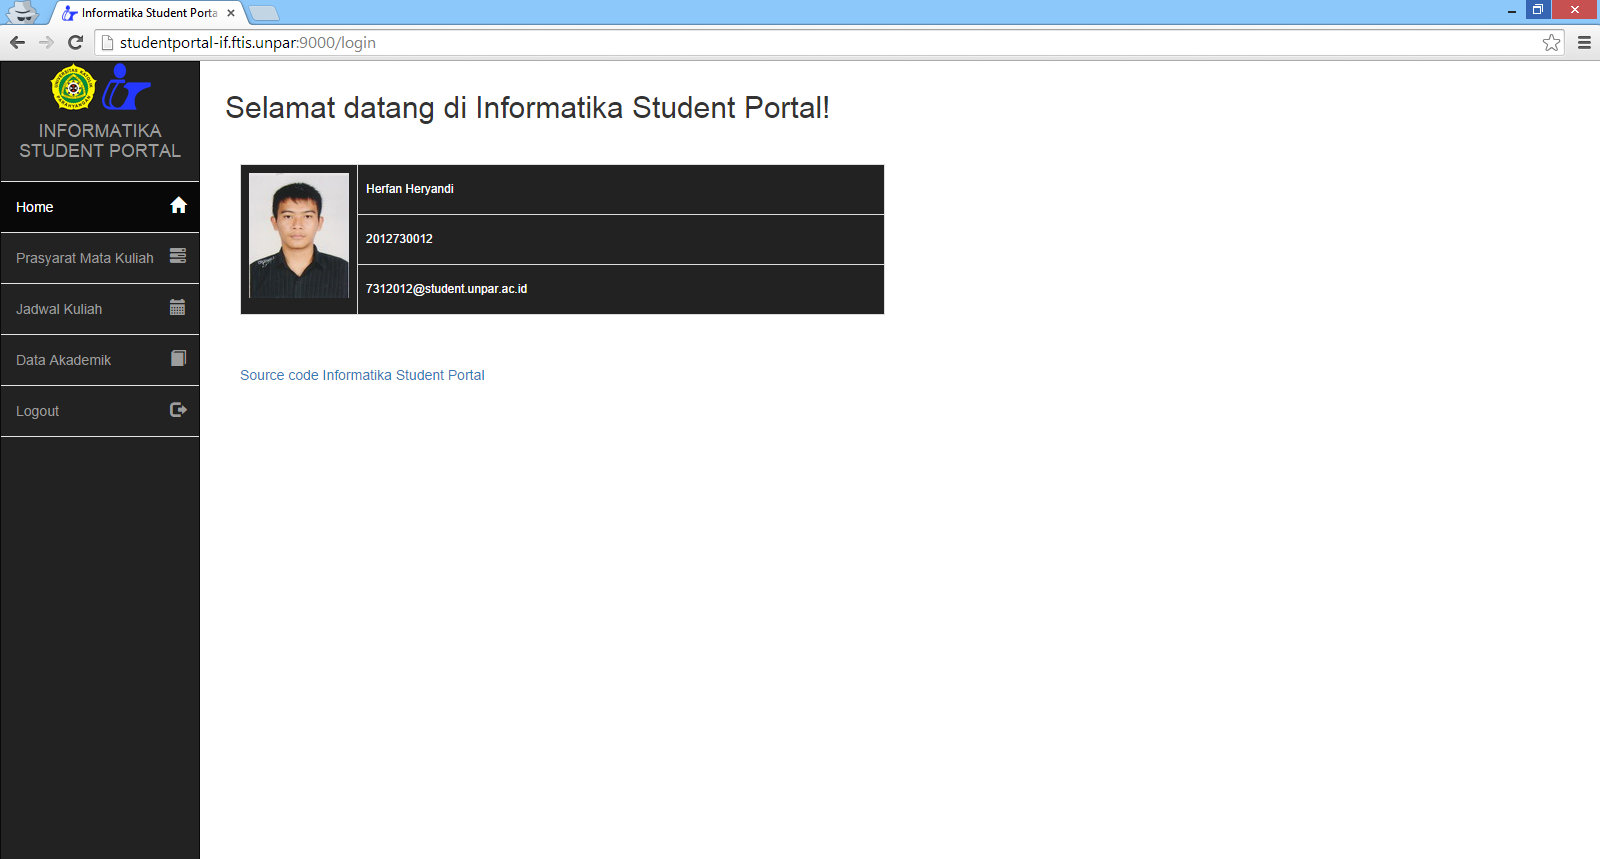
\includegraphics[scale=0.34]{Gambar/hasil_home}
						\caption{Halaman \textit{Home}} 
						\label{fig:5_hasil_utama}
					\end{figure}
						
				\item\textbf{Halaman Prasyarat Mata Kuliah}\\
				Halaman ini menampilkan tabel prasyarat mata kuliah. Jika prasyarat mata kuliah tersedia, pengguna dapat mengklik kode mata kuliah, kemudian akan diarahkan ke kode sumber aturan prasyarat mata kuliah tersebut. Tangkapan layar dari halaman prasyarat mata kuliah dapat dilihat pada Gambar \ref{fig:5_hasil_prasyarat}.
					\begin{figure}[H]
						\centering
						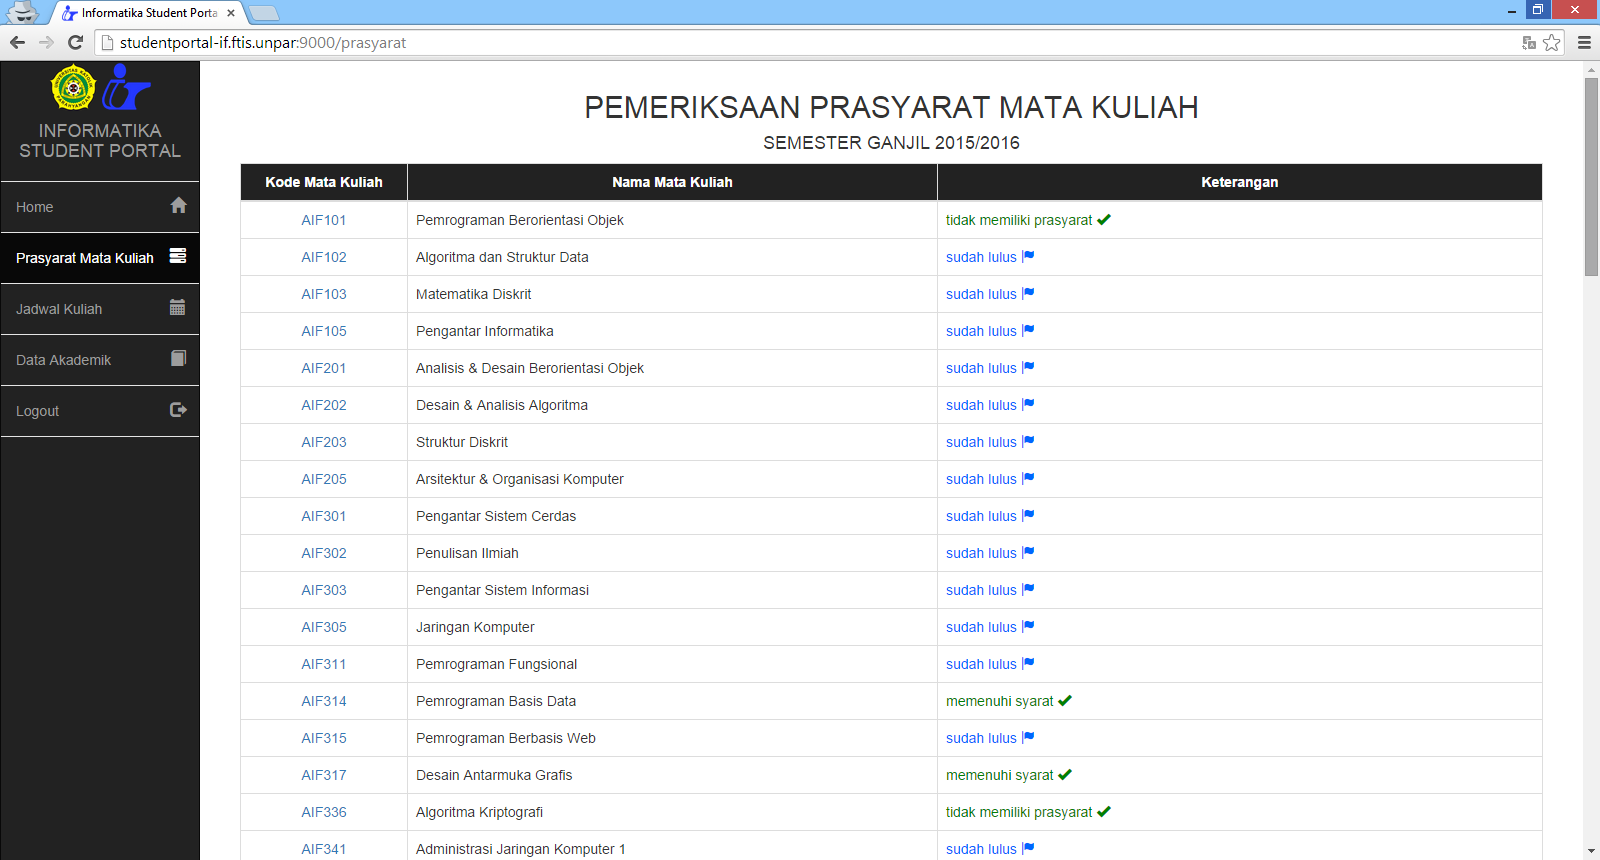
\includegraphics[scale=0.34]{Gambar/hasil_prasyarat}
						\caption{Halaman Prasyarat Mata Kuliah} 
						\label{fig:5_hasil_prasyarat}
					\end{figure}

				\item\textbf{Halaman Jadwal Kuliah}\\
				Halaman ini menampilkan jadwal kuliah yang tersusun dan terurut berdasarkan hari. Tangkapan layar dari halaman jadwal kuliah dapat dilihat pada Gambar \ref{fig:5_hasil_jadwal}. Jika kode mata kuliah diklik, akan muncul \textit{popup} seperti pada Gambar \ref{fig:5_hasil_jadwal_rinci} yang berisi rincian dari jadwal kuliah tersebut.
				\begin{figure}[H]
						\centering
						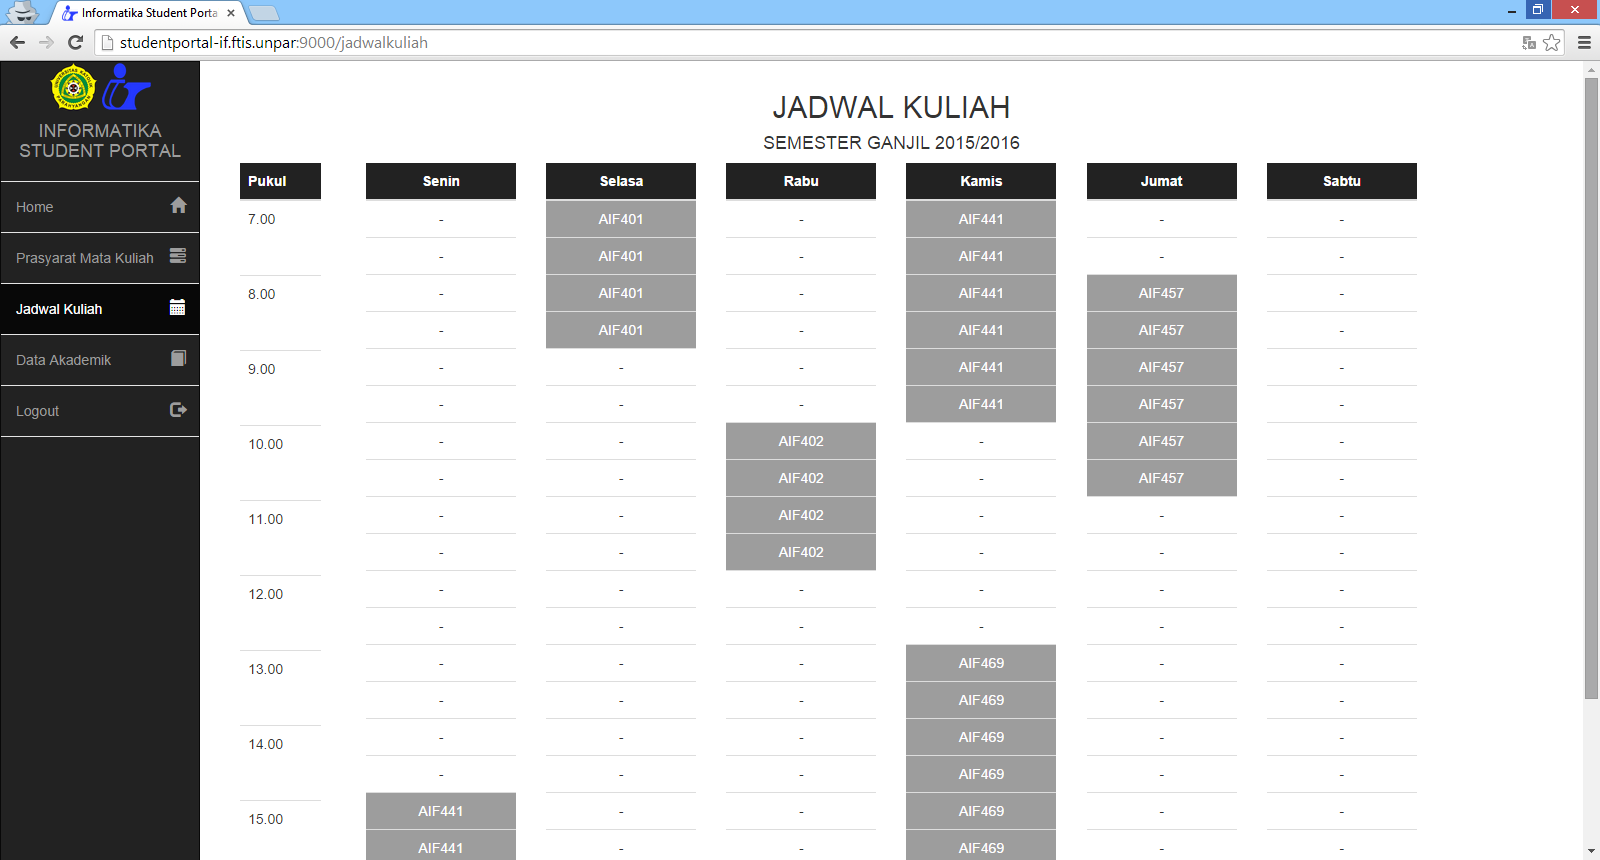
\includegraphics[scale=0.34]{Gambar/hasil_jadwal}
						\caption{Halaman Jadwal Kuliah} 
						\label{fig:5_hasil_jadwal}
					\end{figure}
					
					\begin{figure}[H]
						\centering
						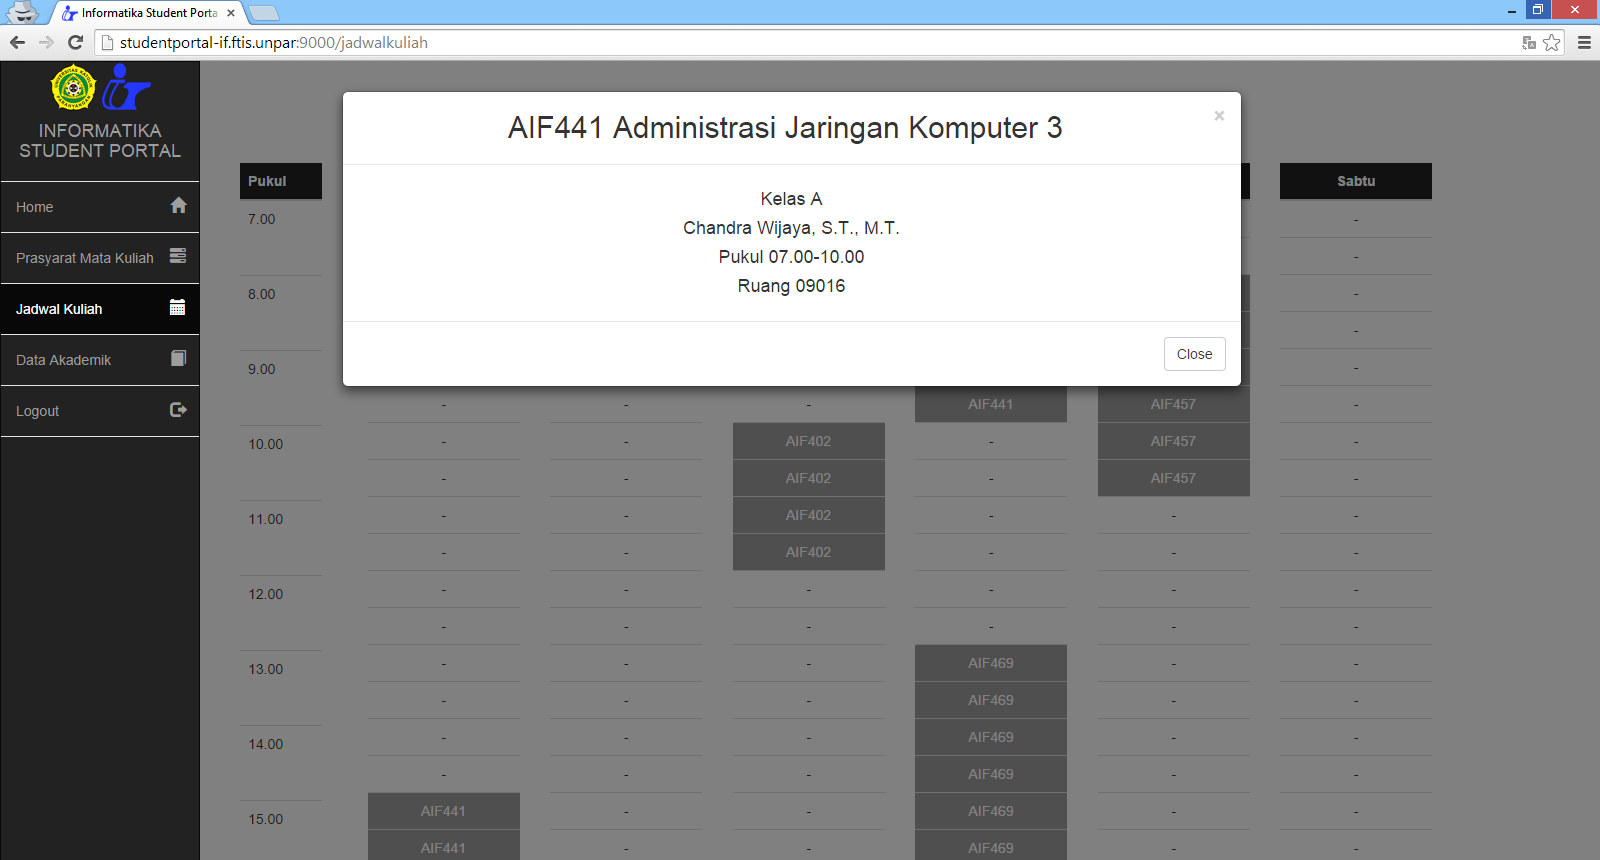
\includegraphics[scale=0.34]{Gambar/hasil_jadwal_popup}
						\caption{Rincian Jadwal Kuliah} 
						\label{fig:5_hasil_jadwal_rinci}
					\end{figure}
					
				\item\textbf{Halaman Data Akademik}\\
				Halaman ini menampilkan data akademik berupa IPS dan IPK yang langsung berubah ketika nilai sudah muncul, sisa SKS, dan status kelulusan mata kuliah pilihan wajib. Tangkapan layar dari halaman data akademik dapat dilihat pada Gambar \ref{fig:5_hasil_ringkasan}.
				\begin{figure}[H]
						\centering
						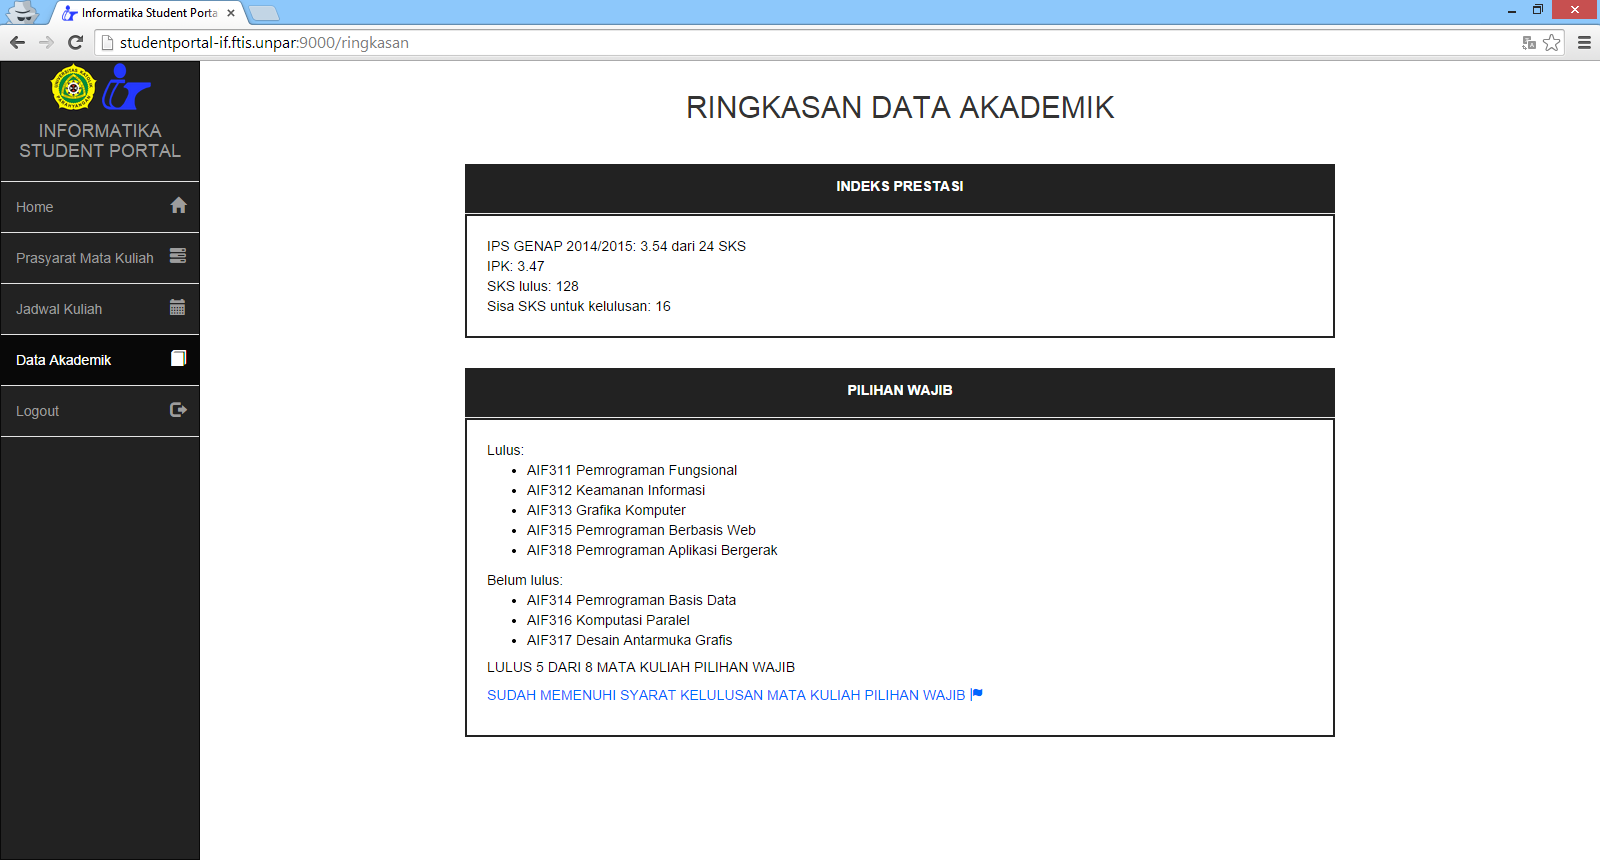
\includegraphics[scale=0.34]{Gambar/hasil_ringkasan}
						\caption{Halaman Data Akademik} 
						\label{fig:5_hasil_ringkasan}
					\end{figure}
			\end{enumerate}
				
\section{Pengujian}
			\subsection{Pengujian Fungsional} 
			Pengujian fungsional dilakukan untuk mengetahui kesesuaian reaksi perangkat lunak dengan reaksi yang diharapkan berdasarkan aksi pengguna terhadap perangkat lunak. Pengujian ini dilakukan pada berbagai sistem yaitu Windows, Linux, MacOS, dan Android dengan hasil yang sama. Terdapat tujuh tes kasus yang diujikan, detail serta hasilnya dapat dilihat pada Tabel \ref{table:hasilFungsional}.
			
			\begin{table}[H]
			\centering
			\caption{Tabel Pengujian Fungsional}
				\begin{tabular}{|p{0.25cm}| p{3.5cm}| p{7cm}| p{2.5cm}|} \hline
				No.	&	Aksi Pengguna	&	Reaksi yang diharapkan	&	Reaksi Perangkat Lunak \\ \hline
				1.	&	Pengguna menjalankan aplikasi	&	Halaman \textit{login} akan ditampilkan	&	sesuai	\\ \hline
				2.	&	Pengguna memasukkan \textit{email} dan \textit{password}	&	Jika \textit{email} dan \textit{password}	sesuai, pengguna akan diarahkan ke halaman utama. & sesuai, namun foto profil tidak muncul jika belum menambahkan eksepsi terhadap sertifikat SSL UNPAR\\ \hline
					&	&	Jika \textit{email} yang dimasukkan bukan \textit{email} \textit{student} UNPAR, akan ditampilkan pesan ``Email tidak valid''&	sesuai	\\ \hline
					&	&	Jika \textit{email} yang dimasukkan bukan \textit{email} mahasiswa teknik informatika, akan ditampilkan pesan ``Maaf, Anda bukan mahasiswa teknik informatika''	&	sesuai	\\ \hline
					&	&	Jika \textit{email} dan \textit{password} tidak sesuai atau mahasiswa bukan mahasiswa aktif, akan ditampilkan pesan ``Password yang Anda masukkan salah atau Anda bukan mahasiswa aktif''	&	sesuai	\\ \hline
				3.	&	Pengguna memilih menu ``Prasyarat Mata Kuliah'' &	Jika pengguna belum memiliki riwayat nilai(masih menempuh semester 1), akan ditampilkan pesan ``PRASYARAT BELUM TERSEDIA''	&	sesuai	\\ \hline
					&	&	Jika pengguna sudah memiliki riwayat nilai	akan ditampilkan tabel prasyarat mata kuliah beserta status pengambilannya &	sesuai	\\ \hline
				4.	&	Pengguna memilih menu ``Jadwal Kuliah'' &	Jika pengguna belum melakukan FRS, cuti studi, atau jadwal kuliah pengguna belum tersedia, akan ditampilkan pesan ``JADWAL KULIAH BELUM TERSEDIA''	&	sesuai	\\ \hline
					&	&	Jika jadwal kuliah pengguna sudah tersedia, akan ditampilkan jadwal kuliah dalam bentuk kalendar yang sudah diurutkan berdasarkan hari &	sesuai	\\ \hline
				5.	&	Pengguna memilih menu ``Data Akademik'' &	Jika pengguna belum memiliki riwayat nilai(masih menempuh semester 1), akan ditampilkan pesan ``DATA AKADEMIK BELUM TERSEDIA'' &	sesuai	\\ \hline
					&	&	Jika pengguna sudah memiliki riwayat nilai, akan ditampilkan ringkasan data akademik mahasiswa berupa IPS semester terakhir, IPK, SKS lulus, sisa SKS kelulusan, dan ringkasan data mengenai mata kuliah pilihan wajib &	sesuai	\\ \hline
				6.	&	Pengguna memilih tombol \textit{logout}	&	Pengguna akan diarahkan kembali ke halaman \textit{login} &	sesuai	\\ \hline
				7.	& Dua pengguna menggunakan aplikasi secara bersamaan	&	Pengguna dapat menggunakan aplikasi dengan akun yang sesuai &	sesuai	\\ \hline
				\end{tabular}
				\label{table:hasilFungsional}
			\end{table}
			
		\subsection{Pengujian Eksperimental} 
		Pengujian eksperimental dilakukan terhadap mahasiswa angkatan 2012 sampai 2015. Dari setiap angkatan, diambil tiga orang untuk melakukan pengujian. Setiap responden diminta untuk melakukan \textit{login} kemudian melihat data dari setiap halaman pada Portal Akademik Mahasiswa dan memastikan apakah data tersebut sudah sesuai dengan data sebenarnya. Responden menolak jika hasil pegujian diperlihatkan dengan alasan privasi, karena itu hasil pengujian dirangkum sebagai berikut:
		\begin{itemize}
			\item Angkatan 2012\\
			Saat melakukan pemeriksaan prasyarat, terdapat mahasiswa dengan status belum lulus mata kuliah ``AIF101 Pemrograman Berorientasi Objek''. Hal ini disebabkan oleh perubahan kurikulum pada tahun 2013. Kode mata kuliah Pemrograman Berorientasi Objek yang sudah ditempuh angkatan 2012 adalah AIF 191. ``AIF191 Pemrograman Berorientasi Objek'' merupakan hasil konversi mata kuliah ``AKS141 Dasar-dasar Pemrograman''\footnote{\url{http://tinyurl.com/lionov}<Kurikulum 2013><ATURAN KONVERSI 
KURIKULUM 2003/2008 ke KURIKLUM 2013>, diakses 25 November 2015}. Hal tersebut sudah ditangani oleh aturan prasyarat SIA Models sehingga tidak mengakibatkan kesalahan pemeriksaan prasyarat mata kuliah. Selain itu, terdapat juga mahasiswa yang pernah cuti studi. Mahasiswa tersebut memiliki mata kuliah ``XCT001 Cuti Studi'' pada riwayat nilai yang tidak memiliki nilai akhir, namun aplikasi yang dibuat sudah dapat menanganinya dengan cara mengabaikan mata kuliah tanpa nilai akhir. Hasil pengujian eksperimental mahasiswa angkatan 2012 sesuai dengan hasil yang diharapkan.
			\item Angkatan 2013\\
			Dalam pengujian terhadap mahasiswa angkatan 2013, terdapat mahasiswa yang pernah melakukan transfer studi. Total SKS lulus dari mahasiswa tersebut tidak sesuai dikarenakan aplikasi hanya menghitung SKS lulus saat dia melakukan perkuliahan di Program Studi Teknik Informatika. Akibatnya, pemeriksaan prasyarat mata kuliah dengan aturan SKS lulus memberikan hasil yang tidak sesuai. Selain itu, IPS, IPK, dan sisa SKS juga memberikan hasil yang tidak sesuai. Hasil pengujian eksperimental mahasiswa angkatan 2013 sesuai dengan hasil yang diharapkan kecuali terhadap mahasiswa yang transfer studi.
			\item Angkatan 2014\\
			Mahasiswa angkatan 2014 belum pernah menempuh mata kuliah pilihan wajib. Pada halaman data akademik, ditampilkan bahwa mata kuliah pilihan wajib yang sudah lulus masih belum ada. Hasil pengujian eksperimental mahasiswa angkatan 2014 sesuai dengan hasil yang diharapkan.
			\item Angkatan 2015\\
			Mahasiswa angkatan 2015 belum memiliki riwayat nilai sehingga belum bisa melihat ringkasan data akademik dan prasyarat mata kuliah. Hasil pengujian eksperimental mahasiswa angkatan 2015 sesuai dengan hasil yang diharapkan.
		\end{itemize}
		